% THIS DOCUMENT IS TAILORED TO REQUIREMENTS FOR SCIENTIFIC COMPUTING.  IT SHOULDN'T
% BE USED FOR NON-SCIENTIFIC COMPUTING PROJECTS
\documentclass[12pt]{article}

\usepackage{amsmath, mathtools}
\usepackage{amsfonts}
\usepackage{amssymb}
\usepackage{graphicx}
\usepackage{colortbl}
\usepackage{xr}
\usepackage{hyperref}
\usepackage{longtable}
\usepackage{xfrac}
\usepackage{tabularx}
\usepackage{float}
\usepackage{siunitx}
\usepackage{booktabs}
\usepackage{caption}
\usepackage{pdflscape}
\usepackage{afterpage}

%\usepackage[round]{natbib}

%\usepackage{refcheck}

\hypersetup{
    bookmarks=true,         % show bookmarks bar?
      colorlinks=true,       % false: boxed links; true: colored links
    linkcolor=red,          % color of internal links (change box color with linkbordercolor)
    citecolor=green,        % color of links to bibliography
    filecolor=magenta,      % color of file links
    urlcolor=cyan           % color of external links
}

%% Comments

\usepackage{color}

\newif\ifcomments\commentstrue %displays comments
%\newif\ifcomments\commentsfalse %so that comments do not display

\ifcomments
\newcommand{\authornote}[3]{\textcolor{#1}{[#3 ---#2]}}
\newcommand{\todo}[1]{\textcolor{red}{[TODO: #1]}}
\else
\newcommand{\authornote}[3]{}
\newcommand{\todo}[1]{}
\fi

\newcommand{\wss}[1]{\authornote{blue}{SS}{#1}} 
\newcommand{\plt}[1]{\authornote{magenta}{TPLT}{#1}} %For explanation of the template
\newcommand{\sjc}[1]{\authornote{cyan}{SC}{#1}}
%% Common Parts

\newcommand{\progname}{Master of Applied Science} 
\newcommand{\authname}{ChemCode
\\ Samuel Crawford}

\usepackage{hyperref}
    \hypersetup{colorlinks=true, linkcolor=blue, citecolor=blue, filecolor=blue,
                urlcolor=blue, unicode=false}
    \urlstyle{same}
                                

% For easy change of table widths
\newcommand{\colZwidth}{1.0\textwidth}
\newcommand{\colAwidth}{0.13\textwidth}
\newcommand{\colBwidth}{0.82\textwidth}
\newcommand{\colCwidth}{0.1\textwidth}
\newcommand{\colDwidth}{0.05\textwidth}
\newcommand{\colEwidth}{0.8\textwidth}
\newcommand{\colFwidth}{0.17\textwidth}
\newcommand{\colGwidth}{0.5\textwidth}
\newcommand{\colHwidth}{0.28\textwidth}

% Used so that cross-references have a meaningful prefix
\newcounter{defnum} %Definition Number
\newcommand{\dthedefnum}{GD\thedefnum}
\newcommand{\dref}[1]{GD\ref{#1}}
\newcounter{datadefnum} %Datadefinition Number
\newcommand{\ddthedatadefnum}{DD\thedatadefnum}
\newcommand{\ddref}[1]{DD\ref{#1}}
\newcounter{theorynum} %Theory Number
\newcommand{\tthetheorynum}{T\thetheorynum}
\newcommand{\tref}[1]{T\ref{#1}}
\newcounter{tablenum} %Table Number
\newcommand{\tbthetablenum}{T\thetablenum}
\newcommand{\tbref}[1]{TB\ref{#1}}
\newcounter{assumpnum} %Assumption Number
\newcommand{\atheassumpnum}{P\theassumpnum}
\newcommand{\aref}[1]{A\ref{#1}}
\newcounter{goalnum} %Goal Number
\newcommand{\gthegoalnum}{P\thegoalnum}
\newcommand{\gsref}[1]{GS\ref{#1}}
\newcounter{instnum} %Instance Number
\newcommand{\itheinstnum}{IM\theinstnum}
\newcommand{\iref}[1]{IM\ref{#1}}
\newcounter{reqnum} %Requirement Number
\newcommand{\rthereqnum}{P\thereqnum}
\newcommand{\rref}[1]{R\ref{#1}}
\newcounter{nfrnum} %NFR Number
\newcommand{\rthenfrnum}{NFR\thenfrnum}
\newcommand{\nfrref}[1]{NFR\ref{#1}}
\newcounter{lcnum} %Likely change number
\newcommand{\lthelcnum}{LC\thelcnum}
\newcommand{\lcref}[1]{LC\ref{#1}}

\usepackage{fullpage}

\newcommand{\deftheory}[9][Not Applicable]
{
\newpage
\noindent \rule{\textwidth}{0.5mm}

\paragraph{RefName: } \textbf{#2} \phantomsection 
\label{#2}

\paragraph{Label:} #3

\noindent \rule{\textwidth}{0.5mm}

\paragraph{Equation:}

#4

\paragraph{Description:}

#5

\paragraph{Notes:}

#6

\paragraph{Source:}

#7

\paragraph{Ref.\ By:}

#8

\paragraph{Preconditions for \hyperref[#2]{#2}:}
\label{#2_precond}

#9

\paragraph{Derivation for \hyperref[#2]{#2}:}
\label{#2_deriv}

#1

\noindent \rule{\textwidth}{0.5mm}

}

\begin{document}

\title{Software Requirements Specification for \progname:\\
A program for solving chemistry problems} 
\author{\authname}
\date{February 3, 2023}
	
\maketitle

~\newpage

\pagenumbering{roman}

\tableofcontents

~\newpage

\section*{Revision History}

\begin{tabularx}{\textwidth}{p{2.5cm}p{1.5cm}X}
\toprule {\bf Date} & {\bf Version} & {\bf Notes}\\
\midrule
Jan. 21, 2023 & 0.0 & Start document, fill in title page, and add references\\
							& 0.1 & Fill in Problem Description and Goal Statements sections, as 
							well as all relevant definitions\\
Jan. 22, 2023 & 0.1.1 & Replace the notion of ``fractional oxidation state'' with
							``nonstoichiometric compound''\\
							& 0.1.2 & Fix capTemplate reference\\
							& 0.1.3 & Update Abbreviations and Acronyms section\\
							& 0.2 & Add IM for balancing a chemical reaction (\iref{balance}), along
							with relevant reference information\\
Jan. 23, 2023 & 0.2.1 & Add IM for determining if a chemical reaction is feasible
							(\iref{feasible}), along with relevant reference information\\
Jan. 25, 2023 & 0.2.2 & Add references between sections for notation and
							definitions\\
							& 0.2.3 & Abstract \iref{feasible}\\
							& 0.2.4 & Add IM for converting chemical equation to a matrix
							(\iref{convert}), along with relevant reference information \\
\bottomrule
\end{tabularx}

~\newpage

\section{Reference Material}

This section records information for easy reference.

\subsection{Table of Units}

Throughout this document SI (Syst\`{e}me International d'Unit\'{e}s) is employed
as the unit system.  In addition to the basic units, several derived units are
used as described below.  For each unit, the symbol is given followed by a
description of the unit and the SI name.
~\newline

\renewcommand{\arraystretch}{1.2}
%\begin{table}[ht]
  \noindent \begin{tabular}{l l l} 
    \toprule		
    \textbf{symbol} & \textbf{unit} & \textbf{SI}\\
    \midrule 
    \si{\metre} & length & metre\\
    \si{\kilogram} & mass	& kilogram\\
    \si{\second} & time & second\\
    \si{\celsius} & temperature & centigrade\\
    \si{\joule} & energy & joule\\
    \si{\watt} & power & watt (W = \si{\joule\per\second})\\
    \bottomrule
  \end{tabular}
  %	\caption{Provide a caption}
%\end{table}

\plt{Only include the units that your SRS actually uses.}

\plt{Derived units, like newtons, pascal, etc, should show their derivation
    (the units they are derived from) if their constituent units are in the
    table of units (that is, if the units they are derived from are used in the
    document).  For instance, the derivation of pascals as
    $\si{\pascal}=\si{\newton\per\square\meter}$ is shown if newtons and m are
    both in the table.  The derivations of newtons would not be shown if kg and
    s are not both in the table.}

\plt{The symbol for units named after people use capital letters, but the name
  of the unit itself uses lower case.  For instance, pascals use the symbol Pa,
  watts use the symbol W, teslas use the symbol T, newtons use the symbol N,
  etc.  The one exception to this is degree Celsius.  Details on writing metric
  units can be found on the 
  \href{https://www.nist.gov/pml/weights-and-measures/writing-metric-units}
  {NIST} web-page.}

\subsection{Table of Symbols}

The table that follows summarizes the symbols used in this document along with
their units.  The choice of symbols was made to be consistent with the heat
transfer literature and with existing documentation for solar water heating
systems.  The symbols are listed in alphabetical order.

\renewcommand{\arraystretch}{1.2}
%\noindent \begin{tabularx}{1.0\textwidth}{l l X}
\noindent \begin{longtable*}{l l p{12cm}} \toprule
\textbf{symbol} & \textbf{unit} & \textbf{description}\\
\midrule 
$A_C$ & \si[per-mode=symbol] {\square\metre} & coil surface area
\\
$A_\text{in}$ & \si[per-mode=symbol] {\square\metre} & surface area over 
which heat is transferred in
\\ 
\bottomrule
\end{longtable*}
\plt{Use your problems actual symbols.  The si package is a good idea to use for
  units.}

\subsection{Abbreviations and Acronyms}

\renewcommand{\arraystretch}{1.2}
\begin{tabular}{l l} 
  \toprule		
  \textbf{symbol} & \textbf{description}\\
  \midrule 
  1D & One-Dimensional\\
  A & Assumption\\
  DD & Data Definition\\
  GD & General Definition\\
  GS & Goal Statement\\
  IM & Instance Model\\
  LC & Likely Change\\
  PS & Physical System Description\\
  R & Requirement\\
  SRS & Software Requirements Specification\\
  T & Theoretical Model\\
  \bottomrule
\end{tabular}\\

\subsection{Mathematical Notation} \label{sec_mathNot}

Matrices are written in bold uppercase letters (for example $\textbf{A}$), while
vectors (1D matrices) are written in bold lowercase letters, (for example
$\textbf{x}$) \cite{osullivan_appendix_2010}. The zero matrix is a special type
of matrix where each element is zero and is represented as $\textbf{0}$
\cite{weisstein_zero_2023}. Individual entries in a matrix are written in
lowercase letters with their row and column number, in that order, written as
subscripts (for example $a_{12}$) \cite{osullivan_appendix_2010}; these
subscripts are sometimes separated by a comma for clarity (for example
$a_{12,34}$) \cite{latecki_matrices_2018}. Two (or more) matrices with the same
number of rows can be joined together to form an ``augmented matrix'', written
as $\left(\textbf{A}\vert \textbf{B}\right)$ \cite{taboga_augmented_2021}.

\plt{If symbols are used to show mathematical operations,
  these should be summarized here.  In some cases the easiest way to summarize
  the notation is to point to a text or other source that explains the
  notation.}

\newpage

\pagenumbering{arabic}

\plt{This SRS template is based on \cite{SmithAndLai2005, SmithEtAl2007}.  It
  will get you started.  You should not modify the section headings, without
  first discussing the change with the course instructor.  Modification means
  you are not following the template, which loses some of the advantage of a
  template, especially standardization.  Although the bits shown below do not
  include type information, you may need to add this information for your
  problem.  If you are unsure, please can ask the instructor.}

\plt{Feel free to change the appearance of the report by modifying the LaTeX
  commands.}

\plt{This template document assumes that a single program is being documented.
  If you are documenting a family of models, you should start with a commonality
  analysis.  A separate template is provided for this.  For program
  families you should look at \cite{Smith2006, SmithMcCutchanAndCarette2017}.
  Single family member programs are often programs based on a single physical
  model.  General purpose tools are usually documented as a family.  Families of
  physical models also come up.}

\plt{The SRS is not generally written, or read, sequentially.  The SRS is a
  reference document.  It is generally read in an ad hoc order, as the need
  arises.  For writing an SRS, and for reading one for the first time, the
  suggested order of sections is:
\begin{itemize}
\item Goal Statement
\item Instance Models
\item Requirements
\item Introduction
\item Specific System Description
\end{itemize}
}

\plt{Guiding principles for the SRS document:
\begin{itemize}
\item Do not repeat the same information at the same abstraction level.  If
  information is repeated, the repetition should be at a different abstraction
  level.  For instance, there will be overlap between the scope section and the
  assumptions, but the scope section will not go into as much detail as the
  assumptions section.
\end{itemize}
}

\plt{The template description comments should be disabled before submitting this
  document for grading.}

\plt{You can borrow any wording from the text given in the template.  It is part
  of the template, and not considered an instance of academic integrity.  Of
  course, you need to cite the source of the template.}

\plt{When the documentation is done, it should be possible to trace back to the
  source of every piece of information.  Some information will come from
  external sources, like terminology.  Other information will be derived, like
  General Definitions.}

\plt{An SRS document should have the following qualities: unambiguous,
  consistent, complete, validatable, abstract and traceable.}

\plt{The overall goal of the SRS is that someone that meets the Characteristics
  of the Intended Reader (Section~\ref{sec_IntendedReader}) can learn,
  understand and verify the captured domain knowledge.  They should not have to
  trust the authors of the SRS on any statements.  They should be able to
  independently verify/derive every statement made.}

\section{Introduction}

\plt{The introduction section is written to introduce the problem.  It starts
  general and focuses on the problem domain. The general advice is to start with
a paragraph or two that describes the problem, followed by a ``roadmap''
paragraph.  A roadmap orients the reader by telling them what sub-sections to
expect in the Introduction section.}

\subsection{Purpose of Document}

\plt{This section summarizes the purpose of the SRS document.  It does not focus
  on the problem itself.  The problem is described in the ``Problem
  Description'' section (Section~\ref{Sec_pd}).  The purpose is for the document
  in the context of the project itself, not in the context of this course.
  Although the ``purpose'' of the document is to get a grade, you should not
  mention this.  Instead, ``fake it'' as if this is a real project.  The purpose
  section will be similar between projects.  The purpose of the document is the
  purpose of the SRS, including communication, planning for the design stage,
  etc.}

\subsection{Scope of Requirements} 

\plt{Modelling the real world requires simplification.  The full complexity of
  the actual physics, chemistry, biology is too much for existing models, and
  for existing computational solution techniques.  Rather than say what is in
  the scope, it is usually easier to say what is not.  You can think of it as
  the scope is initially everything, and then it is constrained to create the
  actual scope.  For instance, the problem can be restricted to 2 dimensions, or
  it can ignore the effect of temperature (or pressure) on the material
  properties, etc.}  

\plt{The scope section is related to the assumptions section
  (Section~\ref{sec_assumpt}).  However, the scope and the assumptions are not
  at the same level of abstraction.  The scope is at a high level.  The focus is
  on the ``big picture'' assumptions.  The assumptions section lists, and
  describes, all of the assumptions.}

\subsection{Characteristics of Intended Reader} \label{sec_IntendedReader}

\plt{This section summarizes the skills and knowledge of the readers of the
  SRS.  It does NOT have the same purpose as the ``User Characteristics''
  section (Section~\ref{SecUserCharacteristics}).  The intended readers are the
  people that will read, review and maintain the SRS.  They are the people that
  will conceivably design the software that is intended to meet the
  requirements.  The user, on the other hand, is the person that uses the
  software that is built.  They may never read this SRS document.  Of course,
  the same person could be a ``user'' and an ``intended reader.''}

\plt{The intended reader characteristics should be written as unambiguously and
  as specifically as possible.  Rather than say, the user should have an
  understanding of physics, say what kind of physics and at what level.  For
  instance, is high school physics adequate, or should the reader have had a
  graduate course on advanced quantum mechanics?}

\subsection{Organization of Document}
This document is based on a template from \cite{smith_captemplate_2022}, which
is itself based on \cite{SmithAndLai2005, SmithEtAl2007}.

\plt{This section provides a roadmap of the SRS document.  It will help the
  reader orient themselves.  It will provide direction that will help them
  select which sections they want to read, and in what order.  This section will
  be similar between project.}

\section{General System Description}

This section provides general information about the system.  It identifies the
interfaces between the system and its environment, describes the user
characteristics and lists the system constraints.  \plt{This text can likely be
  borrowed verbatim.}

\plt{The purpose of this section is to provide general information about the
  system so the specific requirements in the next section will be easier to
  understand. The general system description section is designed to be
  changeable independent of changes to the functional requirements documented in
  the specific system description. The general system description provides a
  context for a family of related models.  The general description can stay the
  same, while specific details are changed between family members.}

\subsection{System Context}

\plt{Your system context will include a figure that shows the abstract view of
  the software.  Often in a scientific context, the program can be viewed
  abstractly following the design pattern of Inputs $\rightarrow$ Calculations
  $\rightarrow$ Outputs.  The system context will therefore often follow this
  pattern.  The user provides inputs, the system does the calculations, and then
  provides the outputs to the user.  The figure should not show all of the
  inputs, just an abstract view of the main categories of inputs (like material
  properties, geometry, etc.).  Likewise, the outputs should be presented from
  an abstract point of view.  In some cases the diagram will show other external
  entities, besides the user.  For instance, when the software product is a
  library, the user will be another software program, not an actual end user.
  If there are system constraints that the software must work with external
  libraries, these libraries can also be shown on the System Context diagram.
  They should only be named with a specific library name if this is required by
  the system constraint.}

\begin{figure}[h!]
\begin{center}
 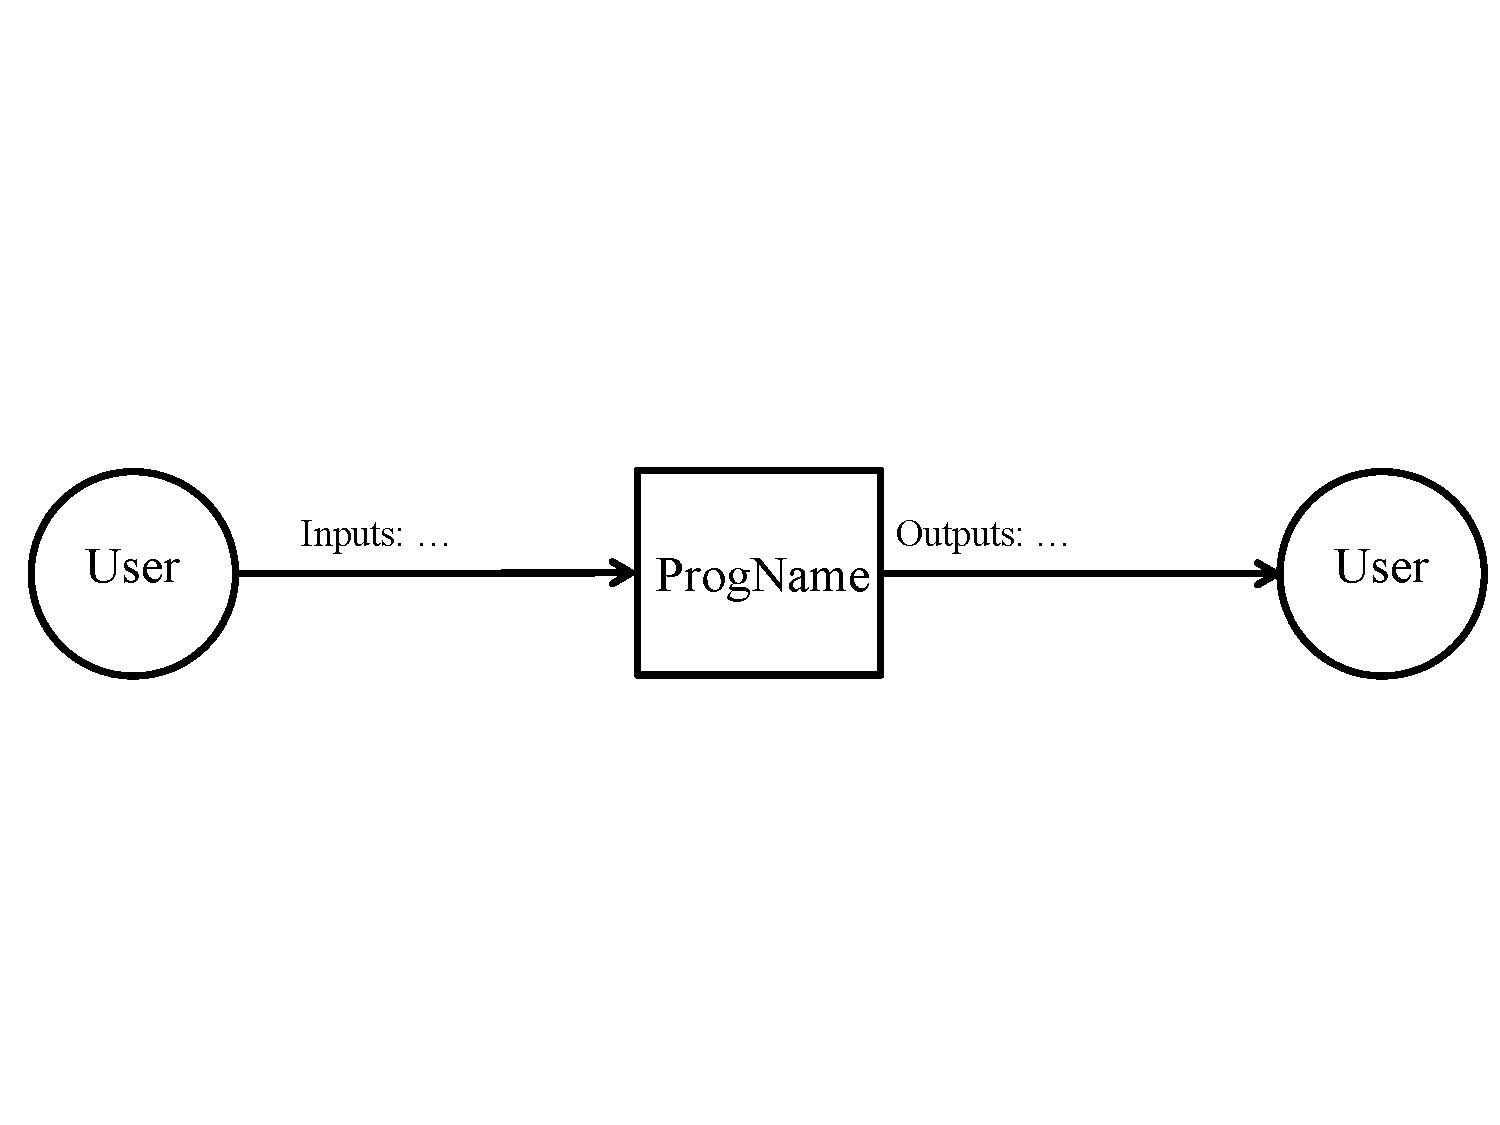
\includegraphics[width=0.6\textwidth]{SystemContextFigure}
\caption{System Context}
\label{Fig_SystemContext} 
\end{center}
\end{figure}

\plt{For each of the entities in the system context diagram its responsibilities
  should be listed.  Whenever possible the system should check for data quality,
  but for some cases the user will need to assume that responsibility.  The list
  of responsibilites should be about the inputs and outputs only, and they
  should be abstract.  Details should not be presented here.  However, the
  information should not be so abstract as to just say ``inputs'' and
  ``outputs''.  A summarizing phrase can be used to characterize the inputs.
  For instance, saying ``material properties'' provides some information, but it
  stays away from the detail of listing every required properties.}

\begin{itemize}
\item User Responsibilities:
\begin{itemize}
\item 
\end{itemize}
\item \progname{} Responsibilities:
\begin{itemize}
\item Detect data type mismatch, such as a string of characters instead of a
  floating point number
\item 
\end{itemize}
\end{itemize}

\subsection{User Characteristics} \label{SecUserCharacteristics}

\plt{This section summarizes the knowledge/skills expected of the user.
  Measuring usability, which is often a required non-function requirement,
  requires knowledge of a typical user.  As mentioned above, the user is a
  different role from the ``intended reader,'' as given in
  Section~\ref{sec_IntendedReader}.  As in Section~\ref{sec_IntendedReader}, the
  user characteristics should be specific an unambiguous.  For instance, ``The
  end user of \progname{} should have an understanding of undergraduate Level 1
  Calculus and Physics.''}

\subsection{System Constraints}

\plt{System constraints differ from other type of requirements because they
  limit the developers' options in the system design and they identify how the
  eventual system must fit into the world. This is the only place in the SRS
  where design decisions can be specified.  That is, the quality requirement for
  abstraction is relaxed here.  However, system constraints should only be
  included if they are truly required.}

\section{Specific System Description}

This section first presents the problem description, which gives a high-level
view of the problem to be solved.  This is followed by the solution characteristics
specification, which presents the assumptions, theories, definitions and finally
the instance models.  \plt{Add any project specific details that are relevant
  for the section overview.}

\subsection{Problem Description} \label{Sec_pd}

\progname{} is intended to balance chemical equations (including ones with
nonstoichiometric compounds; see \nameref{sec_termsDefs}) so
they can be useful for other computations \cite{lund_introduction_2023}.
Additionally, since molecules only exist in whole numbers (since dividing a
molecule changes its composition into new types of molecules), the coefficients
used to balance the equation must be whole
numbers, and by convention should be as small as possible
\cite{lund_introduction_2023}.

\subsubsection{Terminology and  Definitions} \label{sec_termsDefs}
This subsection provides a list of terms that are used in the subsequent
sections and their meaning, with the purpose of reducing ambiguity and making it
easier to correctly understand the requirements:

\begin{itemize}
\item \textbf{Infeasible}: (Referring to a chemical equation) not able to be
balanced \cite{hamid_balancing_2019}.

\item \textbf{Nonstoichiometric Compound}: ``Any solid chemical compound in
which the numbers of atoms of the elements present cannot be expressed as a
ratio of small whole numbers"
\cite{the_editors_of_encyclopaedia_britannica_nonstoichiometric_2010}.

\item \textbf{Product}: A substance created by a chemical reaction
\cite{lund_introduction_2023}.

\item \textbf{Reactant}: A substance present at the beginning of, and involved
in, a chemical reaction \cite{lund_introduction_2023}.

%\item \textbf{Reduced Row Echelon Form}: A form of a matrix where every row
%with only zeros is at the bottom and every column but the rightmost one
%has all zeroes except for one one (which has only zeroes to its left)
%\cite{taboga_reduced_2021}.
\end{itemize}

\subsubsection{Physical System Description} \label{sec_phySystDescrip}

\plt{The purpose of this section is to clearly and unambiguously state the
  physical system that is to be modelled. Effective problem solving requires a
  logical and organized approach. The statements on the physical system to be
  studied should cover enough information to solve the problem. The physical
  description involves element identification, where elements are defined as
  independent and separable items of the physical system. Some example elements
  include acceleration due to gravity, the mass of an object, and the size and
  shape of an object. Each element should be identified and labelled, with their
  interesting properties specified clearly. The physical description can also
  include interactions of the elements, such as the following: i) the
  interactions between the elements and their physical environment; ii) the
  interactions between elements; and, iii) the initial or boundary conditions.}

The physical system of \progname{}, as shown in Figure~?,
includes the following elements:

\begin{itemize}

\item[PS1:] 

\item[PS2:] ...

\end{itemize}

\plt{A figure here makes sense for most SRS documents}

% \begin{figure}[h!]
% \begin{center}
% %\rotatebox{-90}
% {
%  \includegraphics[width=0.5\textwidth]{<FigureName>}
% }
% \caption{\label{<Label>} <Caption>}
% \end{center}
% \end{figure}

\subsubsection{Goal Statements}
Given a representation of a chemical equation, the goal statements 
of \progname{} are:

\begin{itemize}

\item[GS\refstepcounter{goalnum}\thegoalnum \label{G_feasible}:] Determine if
a given chemical reaction is infeasible (see \nameref{sec_termsDefs}).

\item[GS\refstepcounter{goalnum}\thegoalnum \label{G_balance}:] Balance the
inputted chemical equation with the smallest whole number coefficients
possible.

\end{itemize}

\subsection{Solution Characteristics Specification}

\plt{This section specifies the information in the solution domain of the system
  to be developed. This section is intended to express what is required in
  such a way that analysts and stakeholders get a clear picture, and the
  latter will accept it. The purpose of this section is to reduce the problem
  into one expressed in mathematical terms. Mathematical expertise is used to
  extract the essentials from the underlying physical description of the
  problem, and to collect and substantiate all physical data pertinent to the
  problem.}

\plt{This section presents the solution characteristics by successively refining
  models.  It starts with the abstract/general Theoretical Models (TMs) and
  refines them to the concrete/specific Instance Models (IMs).  If necessary
  there are intermediate refinements to General Definitions (GDs).  All of these
  refinements can potentially use Assumptions (A) and Data Definitions (DD).
  TMs are refined to create new models, that are called GMs or IMs. DDs are not
  refined; they are just used. GDs and IMs are derived, or refined, from other
  models. DDs are not derived; they are just given. TMs are also just given, but
  they are refined, not used.  If a potential DD includes a derivation, then
  that means it is refining other models, which would make it a GD or an IM.}

\plt{The above makes a distinction between ``refined'' and ``used.'' A model is
  refined to another model if it is changed by the refinement. When we change a
  general 3D equation to a 2D equation, we are making a refinement, by applying
  the assumption that the third dimension does not matter. If we use a
  definition, like the definition of density, we aren't refining, or changing
  that definition, we are just using it.}

\plt{The same information can be a TM in one problem and a DD in another.  It is
  about how the information is used.  In one problem the definition of
  acceleration can be a TM, in another it would be a DD.}

\plt{There is repetition between the information given in the different chunks
  (TM, GDs etc) with other information in the document.  For instance, the
  meaning of the symbols, the units etc are repeated.  This is so that the
  chunks can stand on their own when being read by a reviewer/user.  It also
  facilitates reuse of the models in a different context.}

\noindent \plt{The relationships between the parts of the document are show in
  the following figure.  In this diagram ``may ref'' has the same role as
  ``uses'' above.  The figure adds ``Likely Changes,'' which are able to
  reference (use) Assumptions.}

\begin{figure}[H]
  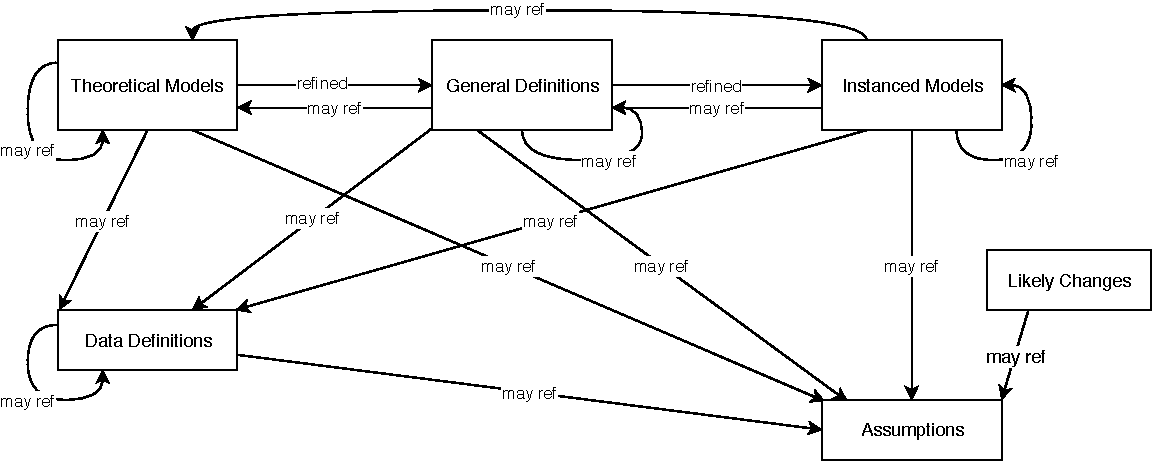
\includegraphics[scale=0.9]{RelationsBetweenTM_GD_IM_DD_A.pdf}
\end{figure}

The instance models that govern \progname{} are presented in
Subsection~\ref{sec_instance}.  The information to understand the meaning of the
instance models and their derivation is also presented, so that the instance
models can be verified.

\subsubsection{Assumptions} \label{sec_assumpt}

\plt{The assumptions are a refinement of the scope.  The scope is general, where
  the assumptions are specific.  All assumptions should be listed, even those
  that domain experts know so well that they are rarely (if ever) written down.}
\plt{The document should not take for granted that the reader knows which
  assumptions have been made. In the case of unusual assumptions, it is
  recommended that the documentation either include, or point to, an explanation
  and justification for the assumption.}

This section simplifies the original problem and helps in developing the
theoretical model by filling in the missing information for the physical
system. The numbers given in the square brackets refer to the theoretical model
[T], general definition [GD], data definition [DD], instance model [IM], or
likely change [LC], in which the respective assumption is used.

\begin{itemize}

\item[A\refstepcounter{assumpnum}\theassumpnum \label{A_meaningfulLabel}:]
  \plt{Short description of each assumption.  Each assumption
    should have a meaningful label.  Use cross-references to identify the
    appropriate traceability to T, GD, DD etc., using commands like dref, ddref
    etc.  Each assumption should be atomic - that is, there should not be an
    explicit (or implicit) ``and'' in the text of an assumption.}

\end{itemize}

\subsubsection{Theoretical Models}\label{sec_theoretical}

\plt{Theoretical models are sets of abstract mathematical equations or axioms
  for solving the problem described in Section ``Physical System Description''
  (Section~\ref{sec_phySystDescrip}). Examples of theoretical models are
  physical laws, constitutive equations, relevant conversion factors, etc.}

This section focuses on the general equations and laws that \progname{} is based
on.  \plt{Modify the examples below for your problem, and add additional models
  as appropriate.}

~\newline

\noindent
\deftheory
% #2 refname of theory
{T:COE}
% #3 label
{Conservation of thermal energy}
% #4 equation
{
  $-{\bf \nabla \cdot q} + g$ = $\rho C \frac{\partial T}{\partial t}$
}
% #5 description
{
  The above equation gives the conservation of energy for transient heat transfer in a material
  of specific heat capacity $C$ (\si{\joule\per\kilogram\per\celsius}) and density $\rho$ 
  (\si{\kilogram\per\cubic\metre}), where $\bf q$ is the thermal flux vector (\si{\watt\per\square\metre}),
  $g$ is the volumetric heat generation
  (\si{\watt\per\cubic\metre}), $T$ is the temperature
  (\si{\celsius}),  $t$ is time (\si{\second}), and $\nabla$ is
  the gradient operator.  For this equation to apply, other forms
  of energy, such as mechanical energy, are assumed to be negligible in the
  system (\aref{A_OnlyThermalEnergy}).  In general, the material properties ($\rho$ and $C$) depend on temperature.
}
% #6 Notes
{
None.
}
% #7 Source
{
  \url{http://www.efunda.com/formulae/heat_transfer/conduction/overview_cond.cfm}
}
% #8 Referenced by
{
  \dref{ROCT}
}
% #9 Preconditions
{
None
}
% #1 derivation - not applicable by default
{}

\plt{``Ref.\ By'' is used repeatedly with the different types of information.
  This stands for Referenced By.  It means that the models, definitions and
  assumptions listed reference the current model, definition or assumption.
  This information is given for traceability.  Ref. By provides a pointer in the
  opposite direction to what we commonly do.  You still need to have a reference
  in the other direction pointing to the current model, definition or
  assumption.  As an example, if T1 is referenced by G2, that means that G2 will
  explicitly include a reference to T1.}

~\newline

\subsubsection{General Definitions}\label{sec_gendef}

\plt{General Definitions (GDs) are a refinement of one or more TMs, and/or of
  other GDs.  The GDs are less abstract than the TMs.  Generally the reduction
  in abstraction is possible through invoking (using/referencing) Assumptions.
  For instance, the TM could be Newton's Law of Cooling stated abstracting.  The
  GD could take the general law and apply it to get a 1D equation.}

This section collects the laws and equations that will be used in building the
instance models.

\plt{Some projects may not have any content for this section, but the section
  heading should be kept.}  \plt{Modify the examples below for your problem, and
  add additional definitions as appropriate.}

~\newline

\noindent
\begin{minipage}{\textwidth}
\renewcommand*{\arraystretch}{1.5}
\begin{tabular}{| p{\colAwidth} | p{\colBwidth}|}
\hline
\rowcolor[gray]{0.9}
Number& GD\refstepcounter{defnum}\thedefnum \label{NL}\\
\hline
Label &\bf Newton's law of cooling \\
\hline
% Units&$MLt^{-3}T^0$\\
% \hline
SI Units&\si{\watt\per\square\metre}\\
\hline
Equation&$ q(t) = h \Delta T(t)$  \\
\hline
Description &
Newton's law of cooling describes convective cooling from a surface.  The law is
stated as: the rate of heat loss from a body is proportional to the difference
in temperatures between the body and its surroundings.
\\
& $q(t)$ is the thermal flux (\si{\watt\per\square\metre}).\\
& $h$ is the heat transfer coefficient, assumed independent of $T$ (\aref{A_hcoeff})
	(\si{\watt\per\square\metre\per\celsius}).\\
&$\Delta T(t)$= $T(t) - T_{\text{env}}(t)$ is the time-dependent thermal gradient
between the environment and the object (\si{\celsius}).
\\
\hline
  Source & Citation here \\
  \hline
  Ref.\ By & \ddref{FluxCoil}, \ddref{FluxPCM}\\
  \hline
\end{tabular}
\end{minipage}\\

\subsubsection*{Detailed derivation of simplified rate of change of temperature}

\plt{This may be necessary when the necessary information does not fit in the
  description field.}
\plt{Derivations are important for justifying a given GD.  You want it to be
  clear where the equation came from.}

\subsubsection{Data Definitions}\label{sec_datadef}

\plt{The Data Definitions are definitions of symbols and equations that are
  given for the problem.  They are not derived; they are simply used by other
  models.  For instance, if a problem depends on density, there may be a data
  definition for the equation defining density.  The DDs are given information
  that you can use in your other modules.}

\plt{All Data Definitions should be used (referenced) by at least one other
  model.}

This section collects and defines all the data needed to build the instance
models. The dimension of each quantity is also given.  \plt{Modify the examples
  below for your problem, and add additional definitions as appropriate.}

~\newline

\noindent
\begin{minipage}{\textwidth}
\renewcommand*{\arraystretch}{1.5}
\begin{tabular}{| p{\colAwidth} | p{\colBwidth}|}
\hline
\rowcolor[gray]{0.9}
Number& DD\refstepcounter{datadefnum}\thedatadefnum \label{FluxCoil}\\
\hline
Label& \bf Heat flux out of coil\\
\hline
Symbol &$q_C$\\
\hline
% Units& $Mt^{-3}$\\
% \hline
  SI Units & \si{\watt\per\square\metre}\\
  \hline
  Equation&$q_C(t) = h_C (T_C - T_W(t))$, over area $A_C$\\
  \hline
  Description & 
                $T_C$ is the temperature of the coil (\si{\celsius}).  $T_W$ is the temperature of the water (\si{\celsius}).  
                The heat flux out of the coil, $q_C$ (\si{\watt\per\square\metre}), is found by
                assuming that Newton's Law 
                of Cooling applies (\aref{A_Newt_coil}).  This law (\dref{NL}) is used on the surface of
                the coil, which has area $A_C$ (\si{\square\metre}) and heat 
                transfer coefficient $h_C$
                (\si{\watt\per\square\metre\per\celsius}).  This equation
                assumes that the temperature of the coil is constant over time (\aref{A_tcoil}) and that it does not vary along the length
                of the coil (\aref{A_tlcoil}).
  \\
  \hline
  Sources& Citation here \\
  \hline
  Ref.\ By & \iref{ewat}\\
  \hline
\end{tabular}
\end{minipage}\\

\subsubsection{Data Types}\label{sec_datatypes}

\plt{This section is optional.  In many scientific computing programs it isn't
  necessary, since the inputs and outpus are straightforward types, like reals,
  integers, and sequences of reals and integers.  However, for some problems it
  is very helpful to capture the type information.}

\plt{The data types are not derived; they are simply stated and used by other
  models.}

\plt{All data types must be used by at least one of the models.}

\plt{For the mathematical notation for expressing types, the recommendation is
  to use the notation of~\cite{HoffmanAndStrooper1995}.}

This section collects and defines all the data types needed to document the
models. \plt{Modify the examples below for your problem, and add additional
  definitions as appropriate.}

~\newline

\noindent
\begin{minipage}{\textwidth}
\renewcommand*{\arraystretch}{1.5}
\begin{tabular}{| p{\colAwidth} | p{\colBwidth}|}
  \hline
  \rowcolor[gray]{0.9}
  Type Name & Name for Type\\
  \hline
  Type Def & mathematical definition of the type\\
  \hline
  Description & description here
  \\
  \hline
  Sources & Citation here, if the type is borrowed from another source\\
  \hline
\end{tabular}
\end{minipage}\\

\subsubsection{Instance Models} \label{sec_instance}    

\plt{The motivation for this section is to reduce the problem defined in
  ``Physical System Description'' (Section~\ref{sec_phySystDescrip}) to one
  expressed in mathematical terms. The IMs are built by refining the TMs and/or
  GDs.  This section should remain abstract.  The SRS should specify the
  requirements without considering the implementation.}

This section transforms the problem defined in Section~\ref{Sec_pd} into 
one which is expressed in mathematical terms. It uses concrete symbols defined 
in Section~\ref{sec_datadef} to replace the abstract symbols in the models 
identified in Sections~\ref{sec_theoretical} and~\ref{sec_gendef}.

The goals \gsref{G_feasible} and \gsref{G_balance} are solved by \iref{feasible}
and \iref{balance}, respectively. 

~\newline

%\noindent
%\begin{minipage}{\textwidth}
%\renewcommand*{\arraystretch}{1.5}
%\begin{tabular}{| p{\colAwidth} | p{\colBwidth}|}
%  \hline
%  \rowcolor[gray]{0.9}
%  Number& IM\refstepcounter{instnum}\theinstnum \label{ewat}\\
%  \hline
%  Label& \bf Energy balance on water to find $T_W$\\
%  \hline
%  Input&$m_W$, $C_W$, $h_C$, $A_C$, $h_P$, $A_P$, $t_\text{final}$, $T_C$, 
%  $T_\text{init}$, $T_P(t)$ from \iref{epcm}\\
%  & The input is constrained so that $T_\text{init} \leq T_C$ (\aref{A_charge})\\
%  \hline
%  Output&$T_W(t)$, $0\leq t \leq t_\text{final}$, such that\\
%  &$\frac{dT_W}{dt} = \frac{1}{\tau_W}[(T_C - T_W(t)) + {\eta}(T_P(t) - T_W(t))]$,\\
%  &$T_W(0) = T_P(0) = T_\text{init}$ (\aref{A_InitTemp}) and $T_P(t)$ from \iref{epcm} \\
%  \hline
%  Description&$T_W$ is the water temperature (\si{\celsius}).\\
%  &$T_P$ is the PCM temperature (\si{\celsius}).\\
%  &$T_C$ is the coil temperature (\si{\celsius}).\\
%  &$\tau_W = \frac{m_W C_W}{h_C A_C}$ is a constant (\si{\second}).\\
%  &$\eta = \frac{h_P A_P}{h_C A_C}$ is a constant (dimensionless).\\
%  & The above equation applies as long as the water is in liquid form,
%  $0<T_W<100^o\text{C}$, where $0^o\text{C}$ and $100^o\text{C}$ are the melting
%  and boiling points of water, respectively (\aref{A_OpRange}, \aref{A_Pressure}).
%  \\
%  \hline
%  Sources& Citation here \\
%  \hline
%  Ref.\ By & \iref{epcm}\\
%  \hline
%\end{tabular}
%\end{minipage}\\
%
%%~\newline
%
%\subsubsection*{Derivation of ...}
%
%\plt{The derivation shows how the IM is derived from the TMs/GDs.  In cases
%  where the derivation cannot be described under the Description field, it will
%  be necessary to include this subsection.}

\noindent
\begin{minipage}{\textwidth}
\renewcommand*{\arraystretch}{1.5}
\begin{tabular}{| p{\colAwidth} | p{\colBwidth}|}
  \hline
  \rowcolor[gray]{0.9}
  Number& IM\refstepcounter{instnum}\theinstnum \label{convert}\\
  \hline
  Label& \bf Matrix representation of elements present in reaction\\
  \hline
  Input& A representation of a chemical equation (see \nameref{sec_termsDefs}).
  \sjc{Constraints?}\\
  \hline
  Output& A matrix such that each entry
  indicates the amount of a given element in a given compound; each row
  corresponds to a different element and each column corresponds to a different
  compound. Positive entries indicate the compound is a reactant (see
  \nameref{sec_termsDefs}), negative
  entries indicate the compound is a product, and zeroes indicate the
  corresponding element is not present in the corresponding compound. \\
  \hline
  Description& N/A
  \\
  \hline
  Sources& \cite{hamid_balancing_2019} \\
  \hline
  Ref.\ By & \iref{feasible}, \iref{balance}\\
  \hline
\end{tabular}
\end{minipage}\\

%~\newline

\subsubsection*{Derivation of ...}

\plt{The derivation shows how the IM is derived from the TMs/GDs.  In cases
  where the derivation cannot be described under the Description field, it will
  be necessary to include this subsection.}
  
\noindent
\begin{minipage}{\textwidth}
\renewcommand*{\arraystretch}{1.5}
\begin{tabular}{| p{\colAwidth} | p{\colBwidth}|}
  \hline
  \rowcolor[gray]{0.9}
  Number& IM\refstepcounter{instnum}\theinstnum \label{feasible}\\
  \hline
  Label& \bf Determination of feasibility\\
  \hline
  Input& $\textbf{A}$ from \iref{convert}\\
%  & The input is constrained so that $T_\text{init} \leq T_C$ (\aref{A_charge})\\
  \hline
  Output& $\textsc{F}$ if $(\textbf{A} \vert \textbf{0})$ has no solutions and 
  			$\textsc{T}$ otherwise\\
  \hline
  Description&$\textbf{A}$ is a matrix representing the amount of each element
  in each compound in a reaction from \iref{convert}. \sjc{Is this necessary?}\\
%  &$\textbf{R}$ is the $m \times n$ matrix $(\textbf{A} \vert \textbf{0})$
%  as close to reduced row echelon form (see \nameref{sec_termsDefs}) as possible
%  from \iref{epcm}.
%	\sjc{Is the relationship between $\textbf{R}$ and $r_{m,n-1}$ clear?}
%  \sjc{Where should $\textbf{R}$ be defined?}\\
  &$\textbf{0}$ is the zero matrix (see \nameref{sec_mathNot}). \\
%  & The above equation applies as long as the water is in liquid form,
%  $0<T_W<100^o\text{C}$, where $0^o\text{C}$ and $100^o\text{C}$ are the melting
%  and boiling points of water, respectively (\aref{A_OpRange}, \aref{A_Pressure}).
%  \\
  \hline
  Sources& \cite{hamid_balancing_2019} \\
%  , \cite{pramoditha_how_2021} \\
  \hline
  Ref.\ By & N/A\\
  \hline
\end{tabular}
\end{minipage}\\

%~\newline

\subsubsection*{Derivation of ...}

\plt{The derivation shows how the IM is derived from the TMs/GDs.  In cases
  where the derivation cannot be described under the Description field, it will
  be necessary to include this subsection.}
  
\noindent
\begin{minipage}{\textwidth}
\renewcommand*{\arraystretch}{1.5}
\begin{tabular}{| p{\colAwidth} | p{\colBwidth}|}
  \hline
  \rowcolor[gray]{0.9}
  Number& IM\refstepcounter{instnum}\theinstnum \label{balance}\\
  \hline
  Label& \bf Calculation of compound coefficients\\
  \hline
  Input& $\textbf{A}$ from \iref{convert}\\
%  & The input is constrained so that $T_\text{init} \leq T_C$ (\aref{A_charge})\\
  \hline
  Output& $\textbf{x}$, such that\\
  &$\textbf{A}\textbf{x} = \textbf{0}$ from \iref{epcm}\\
  \hline
  Description&$\textbf{A}$ is a matrix representing the amount of each element
  in each compound in a reaction from \iref{convert}. \sjc{Is this necessary?}\\
  &$\textbf{x}$ is a vector of coefficients for each compound in the reaction 
  (in the order inputted) so that the equation is balanced.\\
  &$\textbf{0}$ is the zero matrix (see \nameref{sec_mathNot}).\\
%  & The above equation applies as long as the water is in liquid form,
%  $0<T_W<100^o\text{C}$, where $0^o\text{C}$ and $100^o\text{C}$ are the melting
%  and boiling points of water, respectively (\aref{A_OpRange}, \aref{A_Pressure}).
%  \\
  \hline
  Sources& \cite{hamid_balancing_2019} \\
  \hline
  Ref.\ By & N/A\\
  \hline
\end{tabular}
\end{minipage}\\

%~\newline

\subsubsection*{Derivation of ...}

\plt{The derivation shows how the IM is derived from the TMs/GDs.  In cases
  where the derivation cannot be described under the Description field, it will
  be necessary to include this subsection.}

\subsubsection{Input Data Constraints} \label{sec_DataConstraints}    

Table~\ref{TblInputVar} shows the data constraints on the input output
variables.  The column for physical constraints gives the physical limitations
on the range of values that can be taken by the variable.  The column for
software constraints restricts the range of inputs to reasonable values.  The
software constraints will be helpful in the design stage for picking suitable
algorithms.  The constraints are conservative, to give the user of the model the
flexibility to experiment with unusual situations.  The column of typical values
is intended to provide a feel for a common scenario.  The uncertainty column
provides an estimate of the confidence with which the physical quantities can be
measured.  This information would be part of the input if one were performing an
uncertainty quantification exercise.

The specification parameters in Table~\ref{TblInputVar} are listed in
Table~\ref{TblSpecParams}.

\begin{table}[!h]
  \caption{Input Variables} \label{TblInputVar}
  \renewcommand{\arraystretch}{1.2}
\noindent \begin{longtable*}{l l l l c} 
  \toprule
  \textbf{Var} & \textbf{Physical Constraints} & \textbf{Software Constraints} &
                             \textbf{Typical Value} & \textbf{Uncertainty}\\
  \midrule 
  $L$ & $L > 0$ & $L_{\text{min}} \leq L \leq L_{\text{max}}$ & 1.5 \si[per-mode=symbol] {\metre} & 10\%
  \\
  \bottomrule
\end{longtable*}
\end{table}

\noindent 
\begin{description}
\item[(*)] \plt{you might need to add some notes or clarifications}
\end{description}

\begin{table}[!h]
\caption{Specification Parameter Values} \label{TblSpecParams}
\renewcommand{\arraystretch}{1.2}
\noindent \begin{longtable*}{l l} 
  \toprule
  \textbf{Var} & \textbf{Value} \\
  \midrule 
  $L_\text{min}$ & 0.1 \si{\metre}\\
  \bottomrule
\end{longtable*}
\end{table}

\subsubsection{Properties of a Correct Solution} \label{sec_CorrectSolution}

\noindent
A correct solution must exhibit \plt{fill in the details}.  \plt{These
  properties are in addition to the stated requirements.  There is no need to
  repeat the requirements here.  These additional properties may not exist for
  every problem.  Examples include conservation laws (like conservation of
  energy or mass) and known constraints on outputs, which are usually summarized
  in tabular form.  A sample table is shown in Table~\ref{TblOutputVar}}

\begin{table}[!h]
\caption{Output Variables} \label{TblOutputVar}
\renewcommand{\arraystretch}{1.2}
\noindent \begin{longtable*}{l l} 
  \toprule
  \textbf{Var} & \textbf{Physical Constraints} \\
  \midrule 
  $T_W$ & $T_\text{init} \leq T_W \leq T_C$ (by~\aref{A_charge})
  \\
  \bottomrule
\end{longtable*}
\end{table}

\plt{This section is not for test cases or techniques for verification and
  validation.  Those topics will be addressed in the Verification and Validation
  plan.}

\section{Requirements}

\plt{The requirements refine the goal statement.  They will make heavy use of
  references to the instance models.}

This section provides the functional requirements, the business tasks that the
software is expected to complete, and the nonfunctional requirements, the
qualities that the software is expected to exhibit.

\subsection{Functional Requirements}

\noindent \begin{itemize}

\item[R\refstepcounter{reqnum}\thereqnum \label{R_Inputs}:] \plt{Requirements
    for the inputs that are supplied by the user.  This information has to be
    explicit.}

\item[R\refstepcounter{reqnum}\thereqnum \label{R_OutputInputs}:] \plt{It isn't
    always required, but often echoing the inputs as part of the output is a
    good idea.}

\item[R\refstepcounter{reqnum}\thereqnum \label{R_Calculate}:] \plt{Calculation
    related requirements.}

\item[R\refstepcounter{reqnum}\thereqnum \label{R_VerifyOutput}:]
  \plt{Verification related requirements.}

\item[R\refstepcounter{reqnum}\thereqnum \label{R_Output}:] \plt{Output related
    requirements.}

\end{itemize}

\plt{Every IM should map to at least one requirement, but not every requirement
  has to map to a corresponding IM.}

\subsection{Nonfunctional Requirements}

\plt{List your nonfunctional requirements.  You may consider using a fit
  criterion to make them verifiable.}
\plt{The goal is for the nonfunctional requirements to be unambiguous, abstract
  and verifiable.  This isn't easy to show succinctly, so a good strategy may be
to give a ``high level'' view of the requirement, but allow for the details to
be covered in the Verification and Validation document.}
\plt{An absolute requirement on a quality of the system is rarely needed.  For
  instance, an accuracy of 0.0101 \% is likely fine, even if the requirement is
  for 0.01 \% accuracy.  Therefore, the emphasis will often be more on
  describing now well the quality is achieved, through experimentation, and
  possibly theory, rather than meeting some bar that was defined a priori.}
\plt{You do not need an entry for correctness in your NFRs.  The purpose of the
  SRS is to record the requirements that need to be satisfied for correctness.
  Any statement of correctness would just be redundant. Rather than discuss
  correctness, you can characterize how far away from the correct (true)
  solution you are allowed to be.  This is discussed under accuracy.}

\noindent \begin{itemize}

\item[NFR\refstepcounter{nfrnum}\thenfrnum \label{NFR_Accuracy}:]
  \textbf{Accuracy} \plt{Characterize the accuracy by giving the context/use for
    the software.  Maybe something like, ``The accuracy of the computed
    solutions should meet the level needed for $<$engineering or scientific
    application$>$.  The level of accuracy achieved by \progname{} shall be
    described following the procedure given in Section~X of the Verification and
    Validation Plan.''  A link to the VnV plan would be a nice extra.}

\item[NFR\refstepcounter{nfrnum}\thenfrnum \label{NFR_Usability}:] \textbf{Usability}
  \plt{Characterize the usability by giving the context/use for the software.
    You should likely reference the user characteristics section.  The level of
    usability achieved by the software shall be described following the
    procedure given in Section~X of the Verification and Validation Plan.  A
    link to the VnV plan would be a nice extra.}

\item[NFR\refstepcounter{nfrnum}\thenfrnum \label{NFR_Maintainability}:]
  \textbf{Maintainability} \plt{The effort required to make any of the likely
    changes listed for \progname{} should be less than FRACTION of the original
    development time.  FRACTION is then a symbolic constant that can be defined
    at the end of the report.}

\item[NFR\refstepcounter{nfrnum}\thenfrnum \label{NFR_Portability}:]
  \textbf{Portability} \plt{This NFR is easier to write than the others.  The
    systems that \progname{} should run on should be listed here.  When possible
    the specific versions of the potential operating environments should be
    given.  To make the NFR verifiable a statement could be made that the tests
    from a given section of the VnV plan can be successfully run on all of the
    possible operating environments.}

\item Other NFRs that might be discussed include verifiability,
  understandability and reusability.

\end{itemize}

\section{Likely Changes}    

\noindent \begin{itemize}

\item[LC\refstepcounter{lcnum}\thelcnum\label{LC_meaningfulLabel}:] \plt{Give
    the likely changes, with a reference to the related assumption (aref), as appropriate.}

\end{itemize}

\section{Unlikely Changes}    

\noindent \begin{itemize}

\item[LC\refstepcounter{lcnum}\thelcnum\label{LC_meaningfulLabel}:] \plt{Give
    the unlikely changes.  The design can assume that the changes listed will
    not occur.}

\end{itemize}

\section{Traceability Matrices and Graphs}

The purpose of the traceability matrices is to provide easy references on what
has to be additionally modified if a certain component is changed.  Every time a
component is changed, the items in the column of that component that are marked
with an ``X'' may have to be modified as well.  Table~\ref{Table:trace} shows the
dependencies of theoretical models, general definitions, data definitions, and
instance models with each other. Table~\ref{Table:R_trace} shows the
dependencies of instance models, requirements, and data constraints on each
other. Table~\ref{Table:A_trace} shows the dependencies of theoretical models,
general definitions, data definitions, instance models, and likely changes on
the assumptions.

\plt{You will have to modify these tables for your problem.}

\plt{The traceability matrix is not generally symmetric.  If GD1 uses A1, that
  means that GD1's derivation or presentation requires invocation of A1.  A1
  does not use GD1.  A1 is ``used by'' GD1.}

\plt{The traceability matrix is challenging to maintain manually.  Please do
  your best.  In the future tools (like Drasil) will make this much easier.}

\afterpage{
\begin{landscape}
\begin{table}[h!]
\centering
\begin{tabular}{|c|c|c|c|c|c|c|c|c|c|c|c|c|c|c|c|c|c|c|c|}
\hline
	& \aref{A_OnlyThermalEnergy}& \aref{A_hcoeff}& \aref{A_mixed}& \aref{A_tpcm}& \aref{A_const_density}& \aref{A_const_C}& \aref{A_Newt_coil}& \aref{A_tcoil}& \aref{A_tlcoil}& \aref{A_Newt_pcm}& \aref{A_charge}& \aref{A_InitTemp}& \aref{A_OpRangePCM}& \aref{A_OpRange}& \aref{A_htank}& \aref{A_int_heat}& \aref{A_vpcm}& \aref{A_PCM_state}& \aref{A_Pressure} \\
\hline
\tref{T_COE}        & X& & & & & & & & & & & & & & & & & & \\ \hline
\tref{T_SHE}        & & & & & & & & & & & & & & & & & & & \\ \hline
\tref{T_LHE}        & & & & & & & & & & & & & & & & & & & \\ \hline
\dref{NL}           & & X& & & & & & & & & & & & & & & & & \\ \hline
\dref{ROCT}         & & & X& X& X& X& & & & & & & & & & & & & \\ \hline
\ddref{FluxCoil}    & & & & & & & X& X& X& & & & & & & & & & \\ \hline
\ddref{FluxPCM}     & & & X& X& & & & & & X& & & & & & & & & \\ \hline
\ddref{D_HOF}       & & & & & & & & & & & & & & & & & & & \\ \hline
\ddref{D_MF}        & & & & & & & & & & & & & & & & & & & \\ \hline
\iref{ewat}         & & & & & & & & & & & X& X& & X& X& X& & & X \\ \hline
\iref{epcm}         & & & & & & & & & & & & X& X& & & X& X& X& \\ \hline
\iref{I_HWAT}       & & & & & & & & & & & & & & X& & & & & X \\ \hline
\iref{I_HPCM}       & & & & & & & & & & & & & X& & & & & X & \\ \hline
\lcref{LC_tpcm}     & & & & X& & & & & & & & & & & & & & & \\ \hline
\lcref{LC_tcoil}    & & & & & & & & X& & & & & & & & & & & \\ \hline
\lcref{LC_tlcoil}   & & & & & & & & & X& & & & & & & & & & \\ \hline
\lcref{LC_charge}   & & & & & & & & & & & X& & & & & & & & \\ \hline
\lcref{LC_InitTemp} & & & & & & & & & & & & X& & & & & & & \\ \hline
\lcref{LC_htank}    & & & & & & & & & & & & & & & X& & & & \\
\hline
\end{tabular}
\caption{Traceability Matrix Showing the Connections Between Assumptions and Other Items}
\label{Table:A_trace}
\end{table}
\end{landscape}
}

\begin{table}[h!]
\centering
\begin{tabular}{|c|c|c|c|c|c|c|c|c|c|c|c|c|c|c|c|c|c|c|c|c|c|c|c|}
\hline        
	& \tref{T_COE}& \tref{T_SHE}& \tref{T_LHE}& \dref{NL}& \dref{ROCT} & \ddref{FluxCoil}& \ddref{FluxPCM} & \ddref{D_HOF}& \ddref{D_MF}& \iref{ewat}& \iref{epcm}& \iref{I_HWAT}& \iref{I_HPCM} \\
\hline
\tref{T_COE}     & & & & & & & & & & & & & \\ \hline
\tref{T_SHE}     & & & X& & & & & & & & & & \\ \hline
\tref{T_LHE}     & & & & & & & & & & & & & \\ \hline
\dref{NL}        & & & & & & & & & & & & & \\ \hline
\dref{ROCT}      & X& & & & & & & & & & & & \\ \hline
\ddref{FluxCoil} & & & & X& & & & & & & & & \\ \hline
\ddref{FluxPCM}  & & & & X& & & & & & & & & \\ \hline
\ddref{D_HOF}    & & & & & & & & & & & & & \\ \hline
\ddref{D_MF}     & & & & & & & & X& & & & & \\ \hline
\iref{ewat}      & & & & & X& X& X& & & & X& & \\ \hline
\iref{epcm}      & & & & & X& & X& & X& X& & & X \\ \hline
\iref{I_HWAT}    & & X& & & & & & & & & & & \\ \hline
\iref{I_HPCM}    & & X& X& & & & X& X& X& & X& & \\
\hline
\end{tabular}
\caption{Traceability Matrix Showing the Connections Between Items of Different Sections}
\label{Table:trace}
\end{table}

\begin{table}[h!]
\centering
\begin{tabular}{|c|c|c|c|c|c|c|c|}
\hline
	& \iref{ewat}& \iref{epcm}& \iref{I_HWAT}& \iref{I_HPCM}& \ref{sec_DataConstraints}& \rref{R_RawInputs}& \rref{R_MassInputs} \\
\hline
\iref{ewat}            & & X& & & & X& X \\ \hline
\iref{epcm}            & X& & & X& & X& X \\ \hline
\iref{I_HWAT}          & & & & & & X& X \\ \hline
\iref{I_HPCM}          & & X& & & & X& X \\ \hline
\rref{R_RawInputs}     & & & & & & & \\ \hline
\rref{R_MassInputs}    & & & & & & X& \\ \hline
\rref{R_CheckInputs}   & & & & & X& & \\ \hline
\rref{R_OutputInputs}  & X& X& & & & X& X \\ \hline
\rref{R_TempWater}     & X& & & & & & \\ \hline 
\rref{R_TempPCM}       & & X& & & & & \\ \hline
\rref{R_EnergyWater}   & & & X& & & & \\ \hline
\rref{R_EnergyPCM}     & & & & X& & & \\ \hline
\rref{R_VerifyOutput}  & & & X& X& & & \\ \hline
\rref{R_timeMeltBegin} & & X& & & & & \\ \hline
\rref{R_timeMeltEnd}   & & X& & & & & \\ 
\hline
\end{tabular}
\caption{Traceability Matrix Showing the Connections Between Requirements and Instance Models}
\label{Table:R_trace}
\end{table}

The purpose of the traceability graphs is also to provide easy references on
what has to be additionally modified if a certain component is changed.  The
arrows in the graphs represent dependencies. The component at the tail of an
arrow is depended on by the component at the head of that arrow. Therefore, if a
component is changed, the components that it points to should also be
changed. Figure~\ref{Fig_ATrace} shows the dependencies of theoretical models,
general definitions, data definitions, instance models, likely changes, and
assumptions on each other. Figure~\ref{Fig_RTrace} shows the dependencies of
instance models, requirements, and data constraints on each other.

% \begin{figure}[h!]
% 	\begin{center}
% 		%\rotatebox{-90}
% 		{
% 			\includegraphics[width=\textwidth]{ATrace.png}
% 		}
% 		\caption{\label{Fig_ATrace} Traceability Matrix Showing the Connections Between Items of Different Sections}
% 	\end{center}
% \end{figure}


% \begin{figure}[h!]
% 	\begin{center}
% 		%\rotatebox{-90}
% 		{
% 			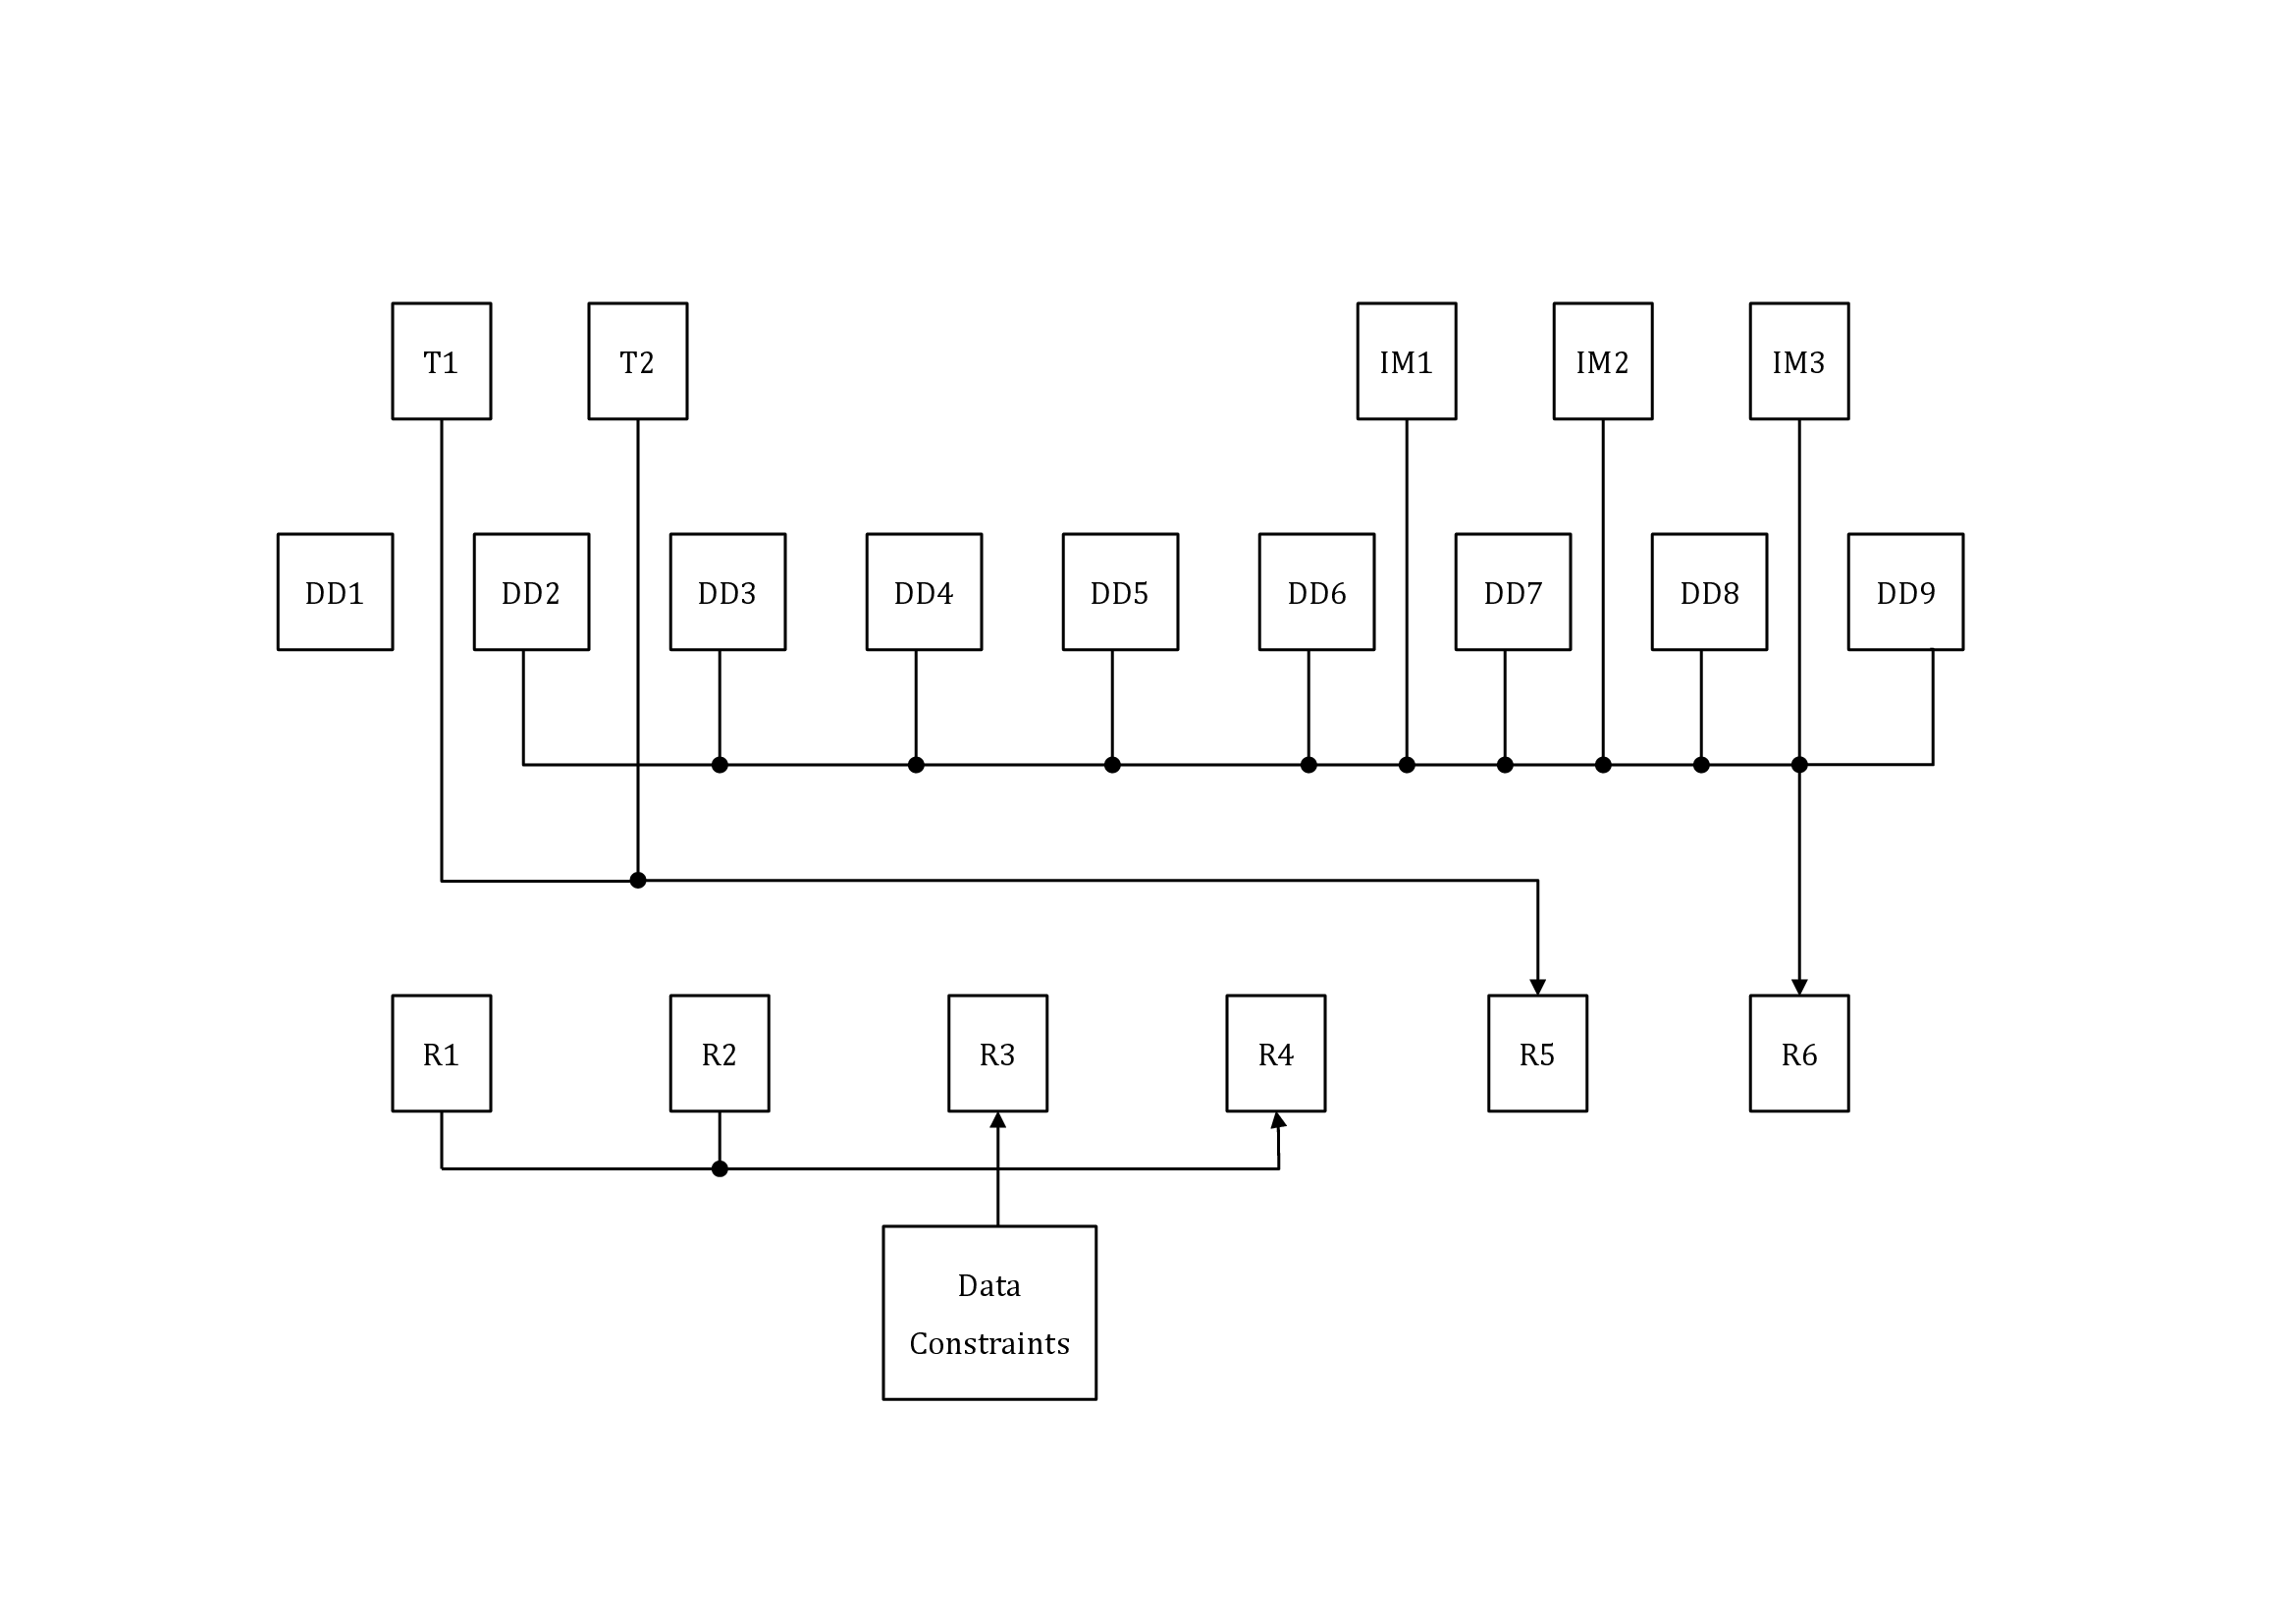
\includegraphics[width=0.7\textwidth]{RTrace.png}
% 		}
% 		\caption{\label{Fig_RTrace} Traceability Matrix Showing the Connections Between Requirements, Instance Models, and Data Constraints}
% 	\end{center}
% \end{figure}

\section{Development Plan}

\plt{This section is optional.  It is used to explain the plan for developing
  the software.  In particular, this section gives a list of the order in which
  the requirements will be implemented.  In the context of a course  this is
  where you can indicate which requirements will be implemented as part of the
  course, and which will be ``faked'' as future work.  This section can be
  organized as a prioritized list of requirements, or it could should the
  requirements that will be implemented for ``phase 1'', ``phase 2'', etc.}

\section{Values of Auxiliary Constants}

\plt{Show the values of the symbolic parameters introduced in the report.}

\plt{The definition of the requirements will likely call for SYMBOLIC\_CONSTANTS.
Their values are defined in this section for easy maintenance.}

\plt{The value of FRACTION, for the Maintainability NFR would be given here.}

\newpage

\bibliographystyle {ieeetr}
\bibliography {../sources}

\newpage

\noindent \plt{The following is not part of the template, just some things to consider
  when filing in the template.}

\noindent \plt{Grammar, flow and \LaTeX advice:
\begin{itemize}
\item For Mac users \texttt{*.DS\_Store} should be in \texttt{.gitignore}
\item \LaTeX{} and formatting rules
\begin{itemize}
\item Variables are italic, everything else not, includes subscripts (link to
  document)
\begin{itemize}
\item \href{https://physics.nist.gov/cuu/pdf/typefaces.pdf}{Conventions}
\item Watch out for implied multiplication
\end{itemize}
\item Use BibTeX
\item Use cross-referencing
\end{itemize}
\item Grammar and writing rules
\begin{itemize}
\item Acronyms expanded on first usage (not just in table of acronyms)
\item ``In order to'' should be ``to''
\end{itemize}
\end{itemize}}

\noindent \plt{Advice on using the template:
\begin{itemize}
\item Difference between physical and software constraints
\item Properties of a correct solution means \emph{additional} properties, not
  a restating of the requirements (may be ``not applicable'' for your problem).
  If you have a table of output constraints, then these are properties of a
  correct solution.
\item Assumptions have to be invoked somewhere
\item ``Referenced by'' implies that there is an explicit reference
\item Think of traceability matrix, list of assumption invocations and list of
  reference by fields as automatically generatable
\item If you say the format of the output (plot, table etc), then your
  requirement could be more abstract
\end{itemize}
}

\newpage{}
\section*{Appendix --- Reflection}

The information in this section will be used to evaluate the team members on the
graduate attribute of Lifelong Learning.  Please answer the following questions:

\begin{enumerate}
  \item What knowledge and skills will the team collectively need to acquire to
  successfully complete this capstone project?  Examples of possible knowledge
  to acquire include domain specific knowledge from the domain of your
  application, or software engineering knowledge, mechatronics knowledge or
  computer science knowledge.  Skills may be related to technology, or writing,
  or presentation, or team management, etc.  You should look to identify at
  least one item for each team member.
  \item For each of the knowledge areas and skills identified in the previous
  question, what are at least two approaches to acquiring the knowledge or
  mastering the skill?  Of the identified approaches, which will each team
  member pursue, and why did they make this choice?
\end{enumerate}

\end{document}